\chapter{Problem Formulation}\label{chap:problem}

\section{Notation and Event Stream Model}
Let $\Omega \subset \mathbb{Z}^2$ denote the pixel grid and $t \in \mathbb{R}_{\ge 0}$ denote continuous time. An event is the tuple
\[
e_i := (x_i, y_i, t_i, p_i) \in \Omega \times \mathbb{R}_{\ge 0} \times \{-1, +1\},
\]
with polarity $p_i$ indicating the sign of the log-intensity change. The event stream over an interval $[0,T]$ is the multiset $E := \{e_i\}_{i=1}^{N(T)}$, where $N(T)$ denotes the number of events observed in $[0,T]$.

We adopt the standard log-intensity threshold model of event generation: a pixel triggers an event when the change in log-intensity exceeds a (per-pixel) contrast threshold $c$; see \cite{Lichtsteiner2008DVS,Brandli2014DAVIS,Posch2014Retinomorphic,Gallego2020Survey}. Following common practice, the stream can be represented as a distribution of impulses at timestamps and locations. Let $u\in\Omega$ denote a pixel coordinate (to avoid conflict with the polarity symbol $p$), and let $\sigma_i := p_i\in\{-1,+1\}$ denote the event polarity. Then an event field $E(u,t)$ integrates Dirac deltas whose amplitudes encode polarity and quantized contrast \cite{Scheerlinck2021Thesis,Wang2025Thesis}:
\begin{equation}
E(u,t) = \sum_{i} \sigma_i\,c\,\delta\!\left(t - t_i\right)\,\mathbf{1}\{u=(x_i,y_i)\}, \qquad \sigma_i \in \{-1,+1\}.
\label{eq:event-field}
\end{equation}
Per-pixel non-idealities (background activity, polarity asymmetry, threshold mismatch, refractory effects) are acknowledged and handled operationally through robust matching tolerances and polarity checks introduced below \cite{Brandli2014DAVIS,Delbruck2020Handbook,Gallego2020Survey}. Timestamp jitter on modern devices is typically small relative to other uncertainties at sub-millisecond horizons \cite{Wang2025Thesis}.

\paragraph{Objective.}
Consistent with the high-level research questions in the introduction, our objective is to identify and \emph{cancel} events that are predictable from a circular-motion model, \emph{asynchronously and per-event}. The aim is to reduce ego-motion clutter early, preserving low latency while leaving residual events that more likely correspond to independent scene/object motion.

\section{Circular-Motion Ego-Motion Model}
Over short horizons, we model the dominant camera motion as planar rotation about an image-plane center $c=(c_x,c_y) \in \mathbb{R}^2$ with signed angular velocity $\omega \in \mathbb{R}$. For $x \in \mathbb{R}^2$, define the rotation of $x$ about $c$ by angle $\theta$ as
\begin{equation}
\mathcal{R}(x; c, \theta) \;=\; c \;+\; R(\theta)\,(x-c),
\qquad
R(\theta) \;=\; 
\begin{bmatrix}\cos \theta & -\sin \theta\\ \sin \theta & \cos \theta\end{bmatrix}.
\label{eq:rot-operator}
\end{equation}
Assuming $\omega$ locally constant over a short prediction horizon $\Delta t$, the \emph{future} location of $x$ is
\begin{equation}
x' \;=\; \mathcal{R}\!\left(x;\, c, \omega\,\Delta t\right).
\label{eq:forward-prop}
\end{equation}
For an event $e_i=(x_i,y_i,t_i,p_i)$ at time $t_i$, write the pixel coordinate as $x_i=(x_i,y_i)$ and denote its forward-predicted location at time $t_i+\Delta t$ as $x_i' = \mathcal{R}(x_i; c, \omega\,\Delta t)$.

\paragraph{Rationale and scope.}
The rotational model is useful beyond the specific rig. (i) It is \emph{depth-free and identifiable}: $(c,\omega)$ is observable from events alone, whereas cancellation with translation generally requires scene depth (or inverse depth) and a richer motion field. (ii) Rotation is a dominant component of hand-held and robotic ego-motion at moderate distances; over short horizons the parallax due to translation is second order relative to the angular term. (iii) The model is analytically compact (two parameters) and widely used for stress-testing event pipelines \cite{Gallego2017Angular,Stoffregen2019Segmentation,Gallego2018CMax}. Our goal is to establish per-event cancellation under a well-posed, low-latency model. Extensions can incorporate constant translational velocity together with an inverse-depth parameterization; we discuss this path and trade-offs in \S\ref{sec:assumptions} and Chapter~\ref{chap:metrics}.

\medskip\noindent\textit{General justification and link to local plane fitting.}
Local motion of a rigid edge under brightness constancy produces approximately \emph{planar} structure in the spatio-temporal volume $(x,y,t)$ over small neighborhoods: events lie near
\( t \approx v_x x + v_y y + d \), where the plane slopes $(v_x,v_y)$ encode image velocity components. This view is agnostic to the global rig and holds for general camera motions. Figure~\ref{fig:plane_fit_xyt} illustrates a least-squares plane fit to a local event cloud, together with $x$--$t$ and $y$--$t$ projections: the fitted plane (and its normal) visualizes how local velocity manifests as slope in $(x,y,t)$. Our rotation-only model specializes this general picture to a depth-free, identifiable field whose parameters $(c,\omega)$ can be estimated reliably at short horizons, making it attractive for causal cancellation.

\medskip\noindent\textit{Why not cancel translation?}
Adding translation is also analytically compact if scene depth (or inverse depth) is available or can be approximated (e.g., far-scene, planar scene). However, translation cancellation requires either per-pixel depth or strong priors, which increases latency/complexity and introduces failure modes under depth discontinuities. Over the short horizons used here, rotation is the dominant contributor to image motion for our apparatus; the translation term is small to first order and is therefore neglected in the cancellation stage. We revisit this assumption and outline extensions under far-scene or weak-translation priors in \S\ref{sec:assumptions}.

\begin{figure}[t]
  \centering
  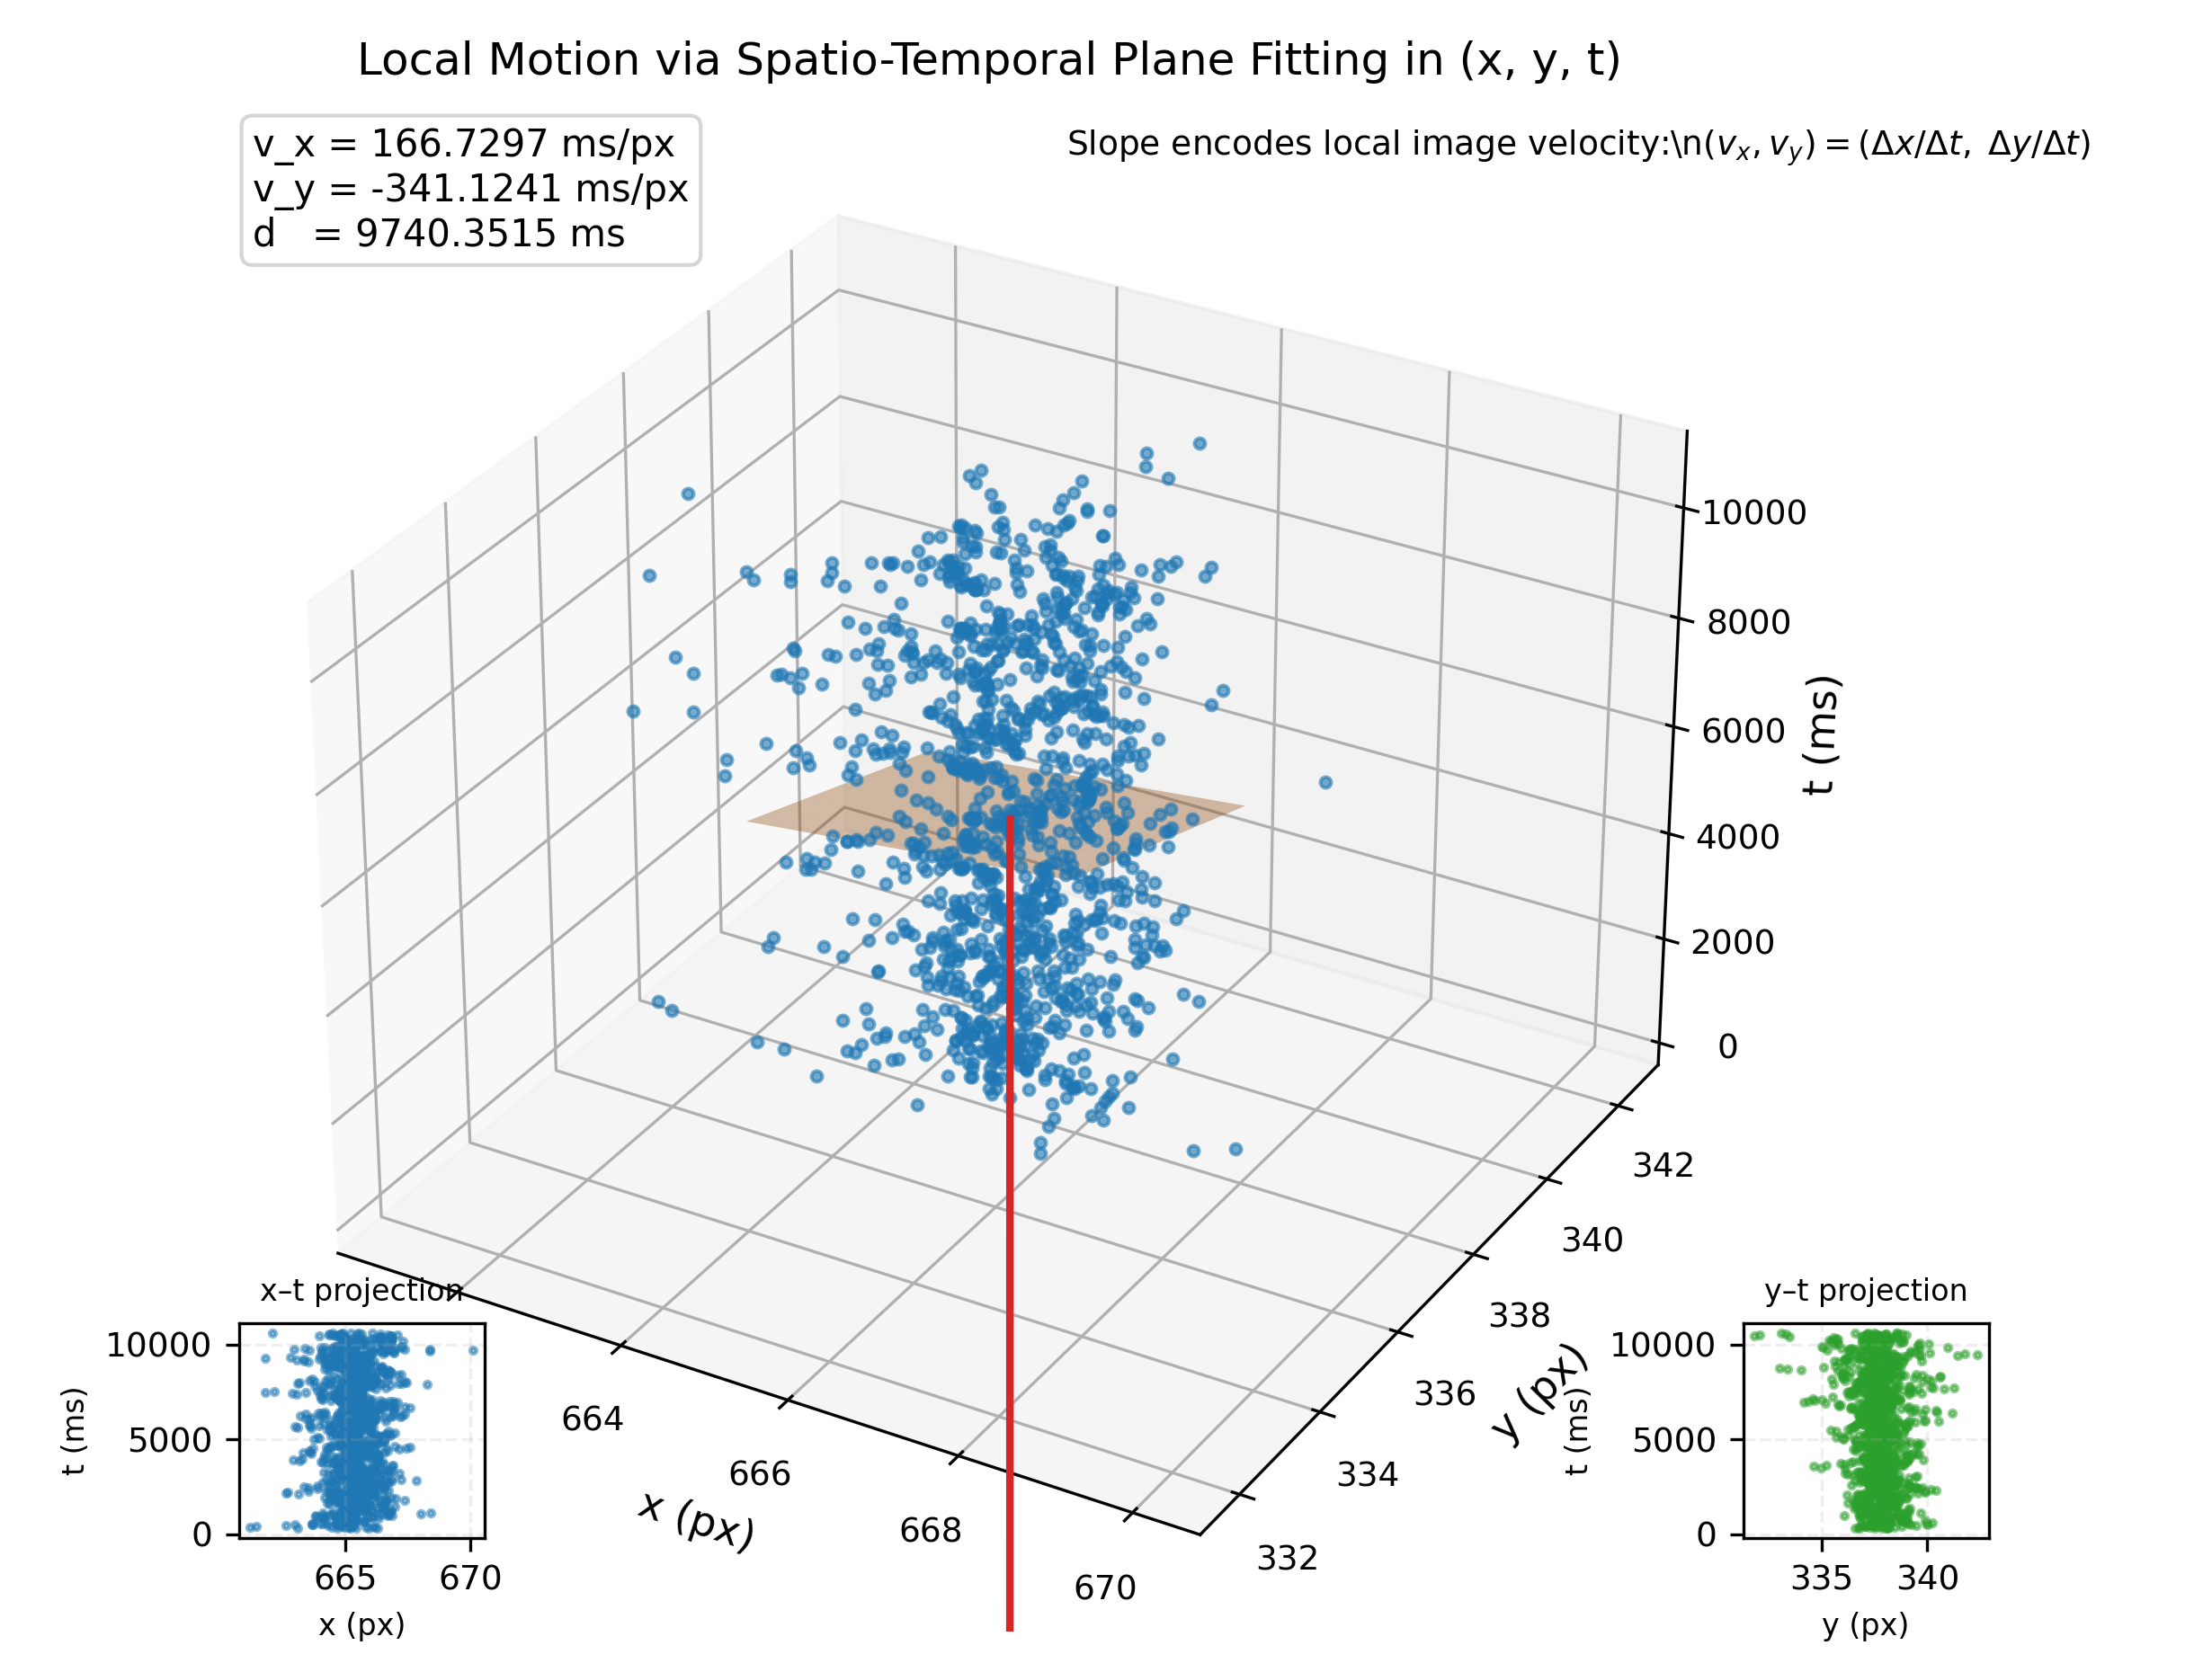
\includegraphics[width=0.88\linewidth]{images/results_figures/plane_fit_xyt.png}
  \caption{Local motion via spatio-temporal plane fitting in $(x,y,t)$. Events from a local patch (scatter) lie near a plane \(t \approx v_x x + v_y y + d\), whose slopes encode image velocity. Insets show $x$--$t$ and $y$--$t$ projections with streaks of slope proportional to velocity. This local model justifies the use of rotational flow as a compact, depth-free specialization for short-horizon cancellation.}
  \label{fig:plane_fit_xyt}
\end{figure}

\section{Per-Event Forward Prediction with a Temporal Gate}\label{sec:temporal_gate}
    We adopt a causal \emph{predict–wait–match} strategy with an explicit temporal tolerance:

\begin{enumerate}
  \item \textbf{Predict.} Upon observing $e_i$ at $t_i$, form the \emph{predicted event}
  \[
  e'_i = (x'_i,\,t'_i,\,p'_i),\quad x'_i=\mathcal{R}(x_i; c, \omega\,\Delta t),\; t'_i=t_i+\Delta t,\; p'_i=-p_i,
  \]
  i.e., the expected location, time and opposite polarity of the cancellable counterpart.
  \item \textbf{Wait.} Defer the decision until the decision time $t^*=t'_i$.
  \item \textbf{Temporal gate.} At $t^*$, compare the single predicted event $e'_i$ against \emph{real} events whose timestamps lie inside a symmetric window:
  \begin{equation}
  \mathcal{N}_t(t^*;\epsilon_t) \;=\; \{\, e_j=(x_j,y_j,t_j,p_j)\in E \,:\, |t_j - t^*| \le \epsilon_t \,\}.
  \label{eq:temporal-window}
  \end{equation}
  \item \textbf{Spatial/polarity gate.} Within $\mathcal{N}_t(t^*;\epsilon_t)$, search for a real event $e_j$ satisfying
  \begin{equation}
  \|x_j - x_i'\|_2 \le \epsilon_{xy},
  \qquad
  \pi(p_i,p_j)=1,
  \label{eq:gating}
  \end{equation}
  where $\epsilon_{xy}>0$ is a spatial tolerance and $\pi$ encodes the polarity rule (default: strict opposite polarity, $\pi(p_i,p_j)=\mathbf{1}\{p_j=-p_i\}$).
\end{enumerate}

If such a match exists, declare $e_i$ \emph{ego-motion predictable} and add $e_i$ to the cancel set; remove both $e_i$ and the matched event $e_j$ from the stream (software-level cancellation). If no match is found inside the spatio-temporal gate, $e_i$ remains in the residual set.

\paragraph{Remarks on implementation.}
Equation~\eqref{eq:temporal-window} enforces a temporal gate with tolerance $\epsilon_t$ (no fixed time bins). In practice, we maintain two time-sorted buffers and advance sliding indices so that, for each $t^*$, we retrieve exactly those real events with $|t - t^*| \le \epsilon_t$ before applying the spatial/polarity test~\eqref{eq:gating}. If $(c,\omega)$ are provided at discrete tracker timestamps, we evaluate $\mathcal{R}(\cdot)$ using parameters interpolated to $t_i$ and $t^*$ (linear or spline), ensuring consistent predictions. The cancellation removes matched pairs from the event stream, preserving causality and low latency without hardware-level interference.

\paragraph{Discussion of polarity.}
Over short intervals, a moving edge driving monotonic log-intensity change tends to produce consistent polarity. We therefore default to \emph{opposite-polarity cancellation} (matching predicted opposite polarity $\bar p_i$ with the real event polarity). When polarity asymmetries are suspected (sensor mismatch), we also evaluate a relaxed polarity policy in sensitivity analyses.

\subsection{Matching Policy and One-to-One Constraints}
Let $\mathcal{N}_t(t^*;\epsilon_t)$ denote the candidate window at decision time. We impose a \emph{one-to-one} pairing between predicted and real events within that window to prevent over-cancellation. A simple and effective policy is \emph{mutual nearest neighbors} within the spatial tolerance: for each real event, find its nearest predicted candidate and vice versa; accept a pair only if both choose each other and~\eqref{eq:gating} holds (polarity included). Greedy distance-ordered matching with a ``used set'' for predicted events is an alternative with similar behavior.

\subsection{Sets, Counters, and Residuals}
Over $[0,T]$, let $E$ denote all observed events, $\mathcal{C}\subseteq E$ the subset declared cancellable under \eqref{eq:temporal-window}--\eqref{eq:gating} and removed via software-level cancellation, and $\mathcal{R} := E \setminus \mathcal{C}$ the \emph{residual} events. Define the \emph{cancellation ratio}
\begin{equation}
\mathrm{CR} \;:=\; \frac{|\mathcal{C}|}{|E|},
\qquad
\mathrm{RR}_\mathcal{A} \;:=\; \frac{|\mathcal{R}\cap \mathcal{A}|}{|\mathcal{A}|}
\label{eq:cr-rr}
\end{equation}
for a region-of-interest $\mathcal{A}\subseteq \Omega\times[0,T]$ (e.g., disc vs.\ background masks). We also report \emph{residual event density} $\rho_\mathcal{A} := \frac{|\mathcal{R}\cap (\Omega_\mathcal{A}\times[0,T])|}{|\Omega_\mathcal{A}|}$ and radial residual profiles on the disc (\S\ref{sec:metrics-bridge}).

\subsection{Causality, Buffers, and Complexity}
The per-event pipeline maintains short spatio-temporal buffers: (i) a small queue of pending predictions indexed by decision times $t^*$; (ii) a time-sorted buffer of real events for the sliding temporal window \eqref{eq:temporal-window}; and (iii) a light spatial index (e.g., grid or k-d tree) for neighborhood queries within radius $\epsilon_{xy}$. All matches are decided using only past and present data at the time of processing (no future timestamps are consulted), preserving causality and low latency (no global batch optimization), similar in spirit to asynchronous processing emphasized in \cite{Wang2025Thesis,Scheerlinck2021Thesis}.

\section{Geometric and Temporal Sensitivity to Model Errors}
Prediction accuracy depends on parameter bias and timing. Let the true parameters be $(c^\star,\omega^\star)$ and the estimates be $(\hat c,\hat\omega)$. Consider an event at radius $r=\|x-c^\star\|_2$ from the true center.

\paragraph{Angular-velocity bias.}
Let $\Delta\omega := \hat\omega-\omega^\star$. Over horizon $\Delta t$, the true angular displacement is $\theta^\star=\omega^\star \Delta t$ and the predicted is $\hat\theta=\hat\omega \Delta t$. The angular error $\delta\theta=\hat\theta-\theta^\star=(\Delta\omega)\Delta t$ induces a spatial prediction error
\begin{equation}
\varepsilon_{\omega}(r,\Delta t) \;=\; \big\|\mathcal{R}(x;c^\star,\hat\theta)-\mathcal{R}(x;c^\star,\theta^\star)\big\|
\;=\; 2r\,\big|\sin(\delta\theta/2)\big|
\;\approx\; r\,|\Delta\omega|\,\Delta t,
\label{eq:angvel-error}
\end{equation}
where the linear approximation holds for small $\delta\theta$.

\paragraph{Center-of-rotation bias.}
Let $\Delta c := \hat c - c^\star$. For small $\Delta t$, the first-order contribution of $\Delta c$ to the spatial error satisfies
\begin{equation}
\varepsilon_{c}(r) \;\lesssim\; \|\Delta c\|_2,
\label{eq:center-error}
\end{equation}
and couples with (\ref{eq:angvel-error}) for general $r$. This bound follows from a first-order expansion of the rotation about a perturbed center: for fixed angular displacement the mapping $x\mapsto c+R(\theta)(x-c)$ is Lipschitz in $c$, hence miscentering by $\Delta c$ produces at most $\mathcal O(\|\Delta c\|_2)$ displacement (triangle inequality), independent of $r$ to first order.

\paragraph{Timing uncertainty, horizon, and the temporal gate.}
To avoid confusion with the polarity symbol $\sigma_i$ used in \eqref{eq:event-field}, we denote effective timing uncertainty by $\tau_t$ (sensor latency variability, timestamp quantization; see hardware timing notes in \cite{Lichtsteiner2008DVS,Delbruck2014ISCAS}). Here, ``phase'' refers to the angular displacement $\theta=\omega\,\Delta t$. Over horizon $\Delta t$, the phase uncertainty is $\sigma_\theta \approx |\omega^\star|\,\tau_t$, contributing spatial uncertainty $\sigma_x \approx r\,\sigma_\theta \approx r\,|\omega^\star|\,\tau_t$. The temporal gate \eqref{eq:temporal-window} explicitly allows $|t_j-t^*|\le \epsilon_t$ so that modest timing error does not cause missed matches. However, increasing $\Delta t$ amplifies phase error via~\eqref{eq:angvel-error}; thus $\Delta t$ trades discriminability (separation in time) against phase robustness.

\paragraph{Implications for the spatial gate.}
A sufficient condition for a match is
\begin{equation}
\varepsilon_{\omega}(r,\Delta t) + \varepsilon_c(r) + \sigma_x \;\le\; \epsilon_{xy},
\label{eq:gate-condition}
\end{equation}
which explains typical cancellation curves: $\mathrm{CR}$ increases with $\epsilon_{xy}$ but saturates/degrades if $\epsilon_{xy}$ is too large (false pairs); and $\mathrm{CR}$ decreases with large $\Delta t$ as phase error grows. These trends motivate the parameter sweeps in Chapter~\ref{chap:metrics}.

\section{Formal Cancellation Rule}
Define the decision indicator
\begin{equation}
\delta(e_i; \hat c,\hat\omega,\Delta t,\epsilon_{xy},\epsilon_t) \;=\;
\begin{cases}
1, & \text{if } \exists\, e_j \in \mathcal{N}_t(t_i+\Delta t;\epsilon_t) \text{ s.t. } \eqref{eq:gating}\text{ holds},\\
0, & \text{otherwise.}
\end{cases}
\label{eq:delta-indicator}
\end{equation}
Then $\mathcal{C}=\{e_i\in E:\delta(e_i;\cdot)=1\}$ and $\mathcal{R}=E\setminus \mathcal{C}$. Rather than posing a global optimization, we study the \emph{sensitivity} of cancellation outcomes to $(\Delta t,\epsilon_{xy},\epsilon_t)$ given $(\hat c,\hat\omega)$ in Chapter~\ref{chap:metrics}, and we report residuals to guard against over-cancellation.

\section{Cancellation Implementation and Representation}
On a successful match, we remove both the originating event $e_i$ and the matched event $e_j$ from the event stream, effectively suppressing the predicted observation in the maintained event representation (e.g., polarity-separated accumulation or voxel grid). This software-level cancellation operates at the decision time $t^*$ with microsecond-scale delay, consistent with asynchronous processing goals \cite{Gallego2018CMax,Bardow2016SOFIE}. In evaluation, matched pairs are simply omitted from downstream processing, avoiding the need for explicit ``anti-event'' data structures.

\section{Assumptions, Limitations, and Threats to Validity}
\label{sec:assumptions}
\textbf{(A1) Static scene.} The background is static; independently moving objects are not modeled by the circular ego-motion and should remain as residuals.

\textbf{(A2) Short-horizon rotation dominance.} Over small $\Delta t$, rotational flow dominates translation for our apparatus; accelerations are small over the horizon. This aligns with rotation-focused practice in event tracking and compensation \cite{Gallego2017Angular,Gallego2018CMax}.

\textbf{(A3) Calibration and warping.} Intrinsics and distortion are pre-compensated or negligible on the ROI; otherwise, normalize coordinates before applying~\eqref{eq:forward-prop}.

\textbf{(A4) Sensor non-idealities.} Background activity, threshold mismatch, polarity asymmetry, and refractory effects are present \cite{Brandli2014DAVIS,Delbruck2020Handbook,Gallego2020Survey}. We mitigate via strict polarity checks, tuned tolerances $(\epsilon_{xy},\epsilon_t)$, and background baselines in the metrics. Timestamp jitter is comparatively minor at our horizons \cite{Wang2025Thesis}.

\textbf{(A5) Causality and bounded memory.} Decisions use only past/present data in short buffers; we avoid global contrast-maximization windows and maintain per-event latency \cite{Bardow2016SOFIE,Gallego2018CMax}.

\paragraph{Failure modes.}
(i) Larger $\Delta t$ and/or angular-velocity bias $\Delta\omega$ cause phase errors (\ref{eq:angvel-error}) and missed matches; (ii) miscentered rotation $\Delta c$ yields radius-dependent residuals; (iii) overly large tolerances over-cancel by matching unrelated events; (iv) flicker can pass spatio-temporal gates unless filtered; (v) pronounced translation or non-circular motion violates the model.

\section{Bridge to Metrics and Experiments}
\label{sec:metrics-bridge}
We quantify performance via: (i) cancellation ratio $\mathrm{CR}$ \eqref{eq:cr-rr}; (ii) residual density $\rho_\mathcal{A}$ on disc vs.\ background masks; (iii) radial residual profiles on the disc; and (iv) sensitivity curves vs.\ $\Delta t$, $\epsilon_{xy}$, $\epsilon_t$, polarity handling, and parameter bias (Chapter~\ref{chap:metrics}). These choices reflect established motion-compensation practice (IWE/contrast) and event-rate diagnostics \cite{Bardow2016SOFIE,Gallego2018CMax,Stoffregen2019Segmentation,Gallego2020Survey}, adapted to proactive per-event cancellation.
